\begin{problem}{/images/problems/30_circle.png}{Points on the circle}
	Find an approximate answer to this question without using integrals and differential equations:
We have a circle with a perimeter of one meter. We randomly select 1369 points in its perimeter. What is the average distance between the two closest points? (Here we mean their distance along the perimeter of the circle, not the Euclidean distance)\\[0.2cm]

Link to the problem on Twitter:  \url{https://twitter.com/Riazi_Cafe/status/1696474726812520522}
\end{problem}
\begin{solution}
The exact answer of the question for $n$ points is equal to $\frac{1}{n^2}$ which is equal to $1/1369^2$ for the case of $1369$ points on the circle.\\[0.2cm]

Because we asked for an approximate answer, below we present a simple $2$-approximate solution to the problem. That is, the number we come up with is within a multiplicative factor of 2 from the exact solution.

We use the double counting technique to get the answer. Let the answer to the question (average distance for the two closest points of $n$ random points on the circle) be equal to $f(n)$. In what follows calculate the probability that by adding an $n+1$th point, the distance between the two nearest points will change.

Our claim is that this probability is between $nf(n)$ and $2nf(n)$.

To show this, let for a particular arrangement $A$ the distance between the two nearest points be equal to $f(n,A)$.
For each of the $n$ points, we color an arc of the circle whose distance from that point (along the circle's perimeter) is equal to $f(n,A)$.
We color the counter-clockwise part of the arc with blue and the clockwise part of the arc with red.
Because $f(n,A)$ is equal to the distance of the closest two points, then all the blue arcs are disjoint.
Also, so are all of the red arcs.
However, red and blue arcs may overlap.

Therefore, the total size of all colored arcs is between
$nf(n,A)$
and
$2nf(n,A)$.

\begin{center}
	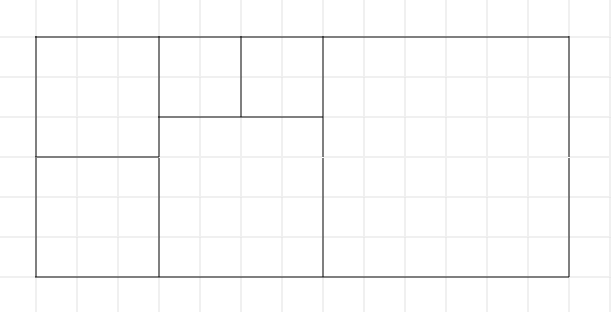
\includegraphics[width=9cm]{/images/problems/sol1.png}
\end{center}

Keep in mind that the perimeter of the circle is 1, and thus if the $n+1$th point is added, the probability that it will be placed on a colored arc is between
$n f(n,A)$
and
$2nf(n,A)$.

If we calculate the average of this probability for all configurations $A$ of the first $n$ points, this probability would be between
$nf(n)$
and $2nf(n)$.  Notice that this is exactly equal to the probability that by adding the $n+1$'th point, the distance between the two closest points change.

Now we calculate the same quantity in another way.
Since all $n+1$ points placed on the circle are random, then the probability that any point is one of the ends of the closest two points is equal to
$2/(n+1)$.

Thus we have $2/(n+1) \geq n\cdot f(n)$ and $2/(n+1) \leq 2n\cdot f(n)$ which together imply $\frac{1}{n\cdot(n+1)} \leq f(n) \leq \frac{2}{n\cdot(n+1)}$

\end{solution}